\newcommand\tab[1][1cm]{\hspace*{#1}}
\graphicspath{ {images/} }
\paragraph{Informatii generale}
\begin{itemize}
\item


	\tab Proiectul consta in proiectarea unui robot multifunctional bazat peplacile de dezvoltare Arduino. Robotul experimental este alcatuit din urmatoarele componente:\\
-	Placa microcontroller compatibila Arduino Uno;\\
-	Driver motoare L298N Dual H-Bridge;\\
-	2x Motor DC;\\
-	1 Motor Servo;\\
-	Carcasa baterii 4x AA (R6);\\
-	2 roti conectate la motoare, 1 roata suport;\\
-	Suport plexiglas;\\
-	Doua placi de prototipizare (BreadBoard)\\
-	1 senzor sonar;\\

	\begin{center}
	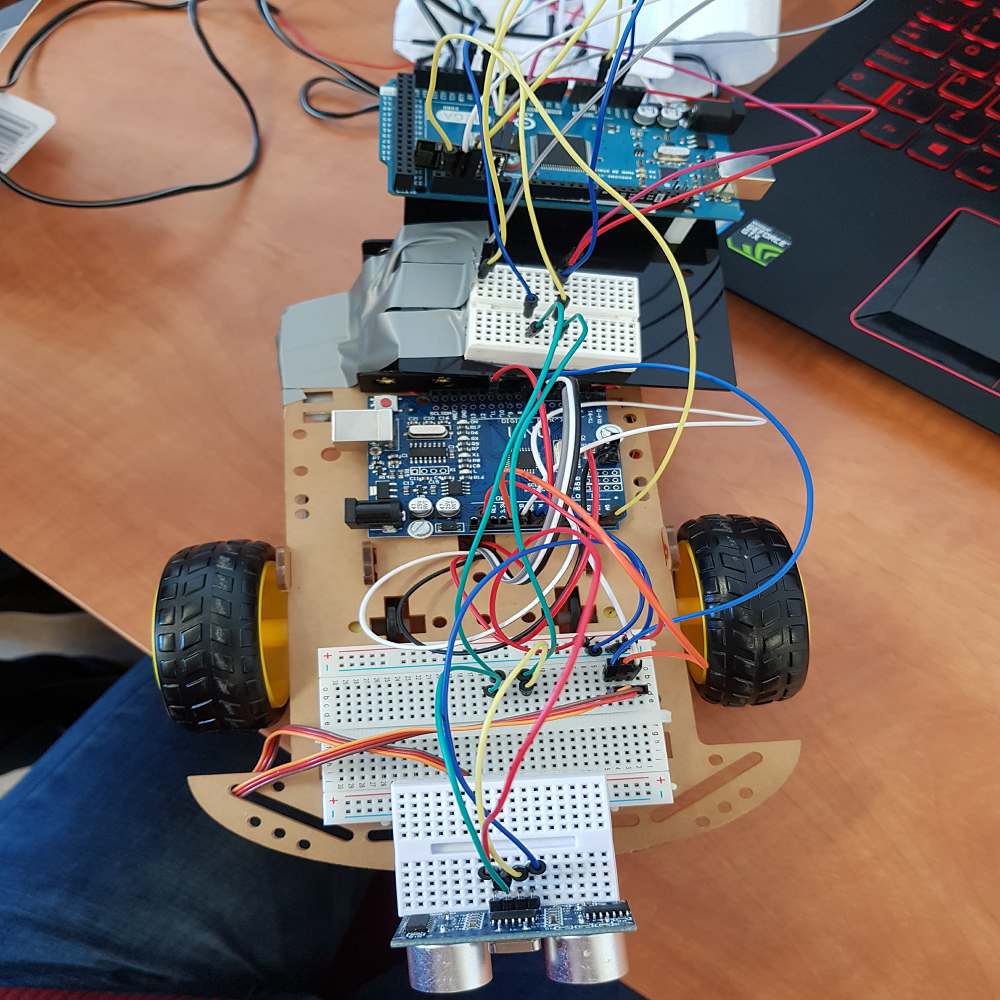
\includegraphics[scale=0.5]{robo22.png}\\
	\end{center}
\end{itemize}

\paragraph{\bf{Functionalitati}}
\begin{itemize}
\item
	\tab In urma realizarii proiectului, robotul experimental dipune de urmatoarele functionalitati:\\
•	Detectia si ocolirea obstacolelor: functionalite posibila datorita utilizarii senzorului sonar, care alaturi de motorul servo determina distanta si unghiul pana la obstacole sau spre spatiul liber.\\
•	Harta a mediului inconjurator:  detectarea de obstacole pentru pozitionarea acestora pe harta.\\
•	Transmiterea datelor utillizand modulul wifi.\\

	\tab O caracteristica importanta a robotului consta in tranzitia implementarii functionalitatilor principale de pe placa Arduino Uno pe placa de dezvoltarea Arduino Mega2560. Astfel, logica de functionare a motoarelor DC si a motorului servo ramane in continuare in seama placii Ardino UNO, pe cand restul functionalitatilor sunt implementate de catre Arduino Mega2560 prin utilizarea protocolului I2C ( Inter Integrated Circuit). \\
	\tab Protocolul I2C reprezinta un protocol ce a fost creat pentru a permite mai multor circuite integrate “slave” sa comunice cu unul sau mai multe cipuri “master”.  Astfel, rolul de “master” este reprezentat de placa  Arduino Mega2560, iar rolul de “slave” este reprezentat de placa Arduino UNO.\\

\end{itemize}